%OL Tracking Usage Instructions

\documentclass[12pt,letterpaper,oneside]{report}
\usepackage[bookmarks=true]{hyperref}
\usepackage[pdftex]{graphicx}
\usepackage[small]{caption}
\usepackage[small]{caption}
\usepackage[final]{pdfpages}
\usepackage{float}
\usepackage{winfonts}
\renewcommand{\thesection}{\arabic{section}}
%
%  definitions.tex
%

%\usepackage{showkeys}

%\usepackage{mathptmx}
\usepackage{amsmath}
\usepackage{multicol}
\usepackage{multirow}
\usepackage{subfigure}
\usepackage{graphicx}
\usepackage{abbrevs}
\usepackage{lips}
\usepackage{gensymb}
\usepackage{type1cm}
\usepackage{type1ec}
%\usepackage{natbib}



% Fancy verbatim package and listings - they work together well to include code
\usepackage{fancyvrb}
\fvset{fontsize=\scriptsize,resetmargins=true,tabsize=4,baselinestretch=1,numbers=left,stepnumber=5}
\usepackage{listings}
\lstset{showstringspaces=true,breaklines=true,tabsize=4,prebreak=\mbox{$\swarrow$},breakautoindent=false,fancyvrb=true}

% Pretty numbers
\usepackage[np,autolanguage]{numprint}
\makeatletter
\renewcommand*\nprt@dotlist{.}
\renewcommand*\nprt@ignorelist{,}
\g@addto@macro\npstyleenglish{%
 \npthousandsep{\,}%
}%
\makeatother

% URLs
\usepackage{url}

% For the array package, define new column types and some shortcuts
\usepackage{array}
\newcommand{\PreserveBackslash}[1]{\let\temp=\\#1\let\\=\temp}
\let\PBS=\PreserveBackslash
\newcolumntype{C}{>{$}c<{$}}
\newcolumntype{R}{>{$}r<{$}}
\newcolumntype{L}{>{$}l<{$}}

\usepackage{microtype}



\begin{document}
\title{OL Tracking: Code Usage Instructions\\v 2.0}
\author{Ulvi Acikoz}
\date{July 7, 2011}
\maketitle
\newpage
\pagenumbering{roman}
\tableofcontents
\newpage
\listoftables
\newpage
\pagenumbering{arabic}
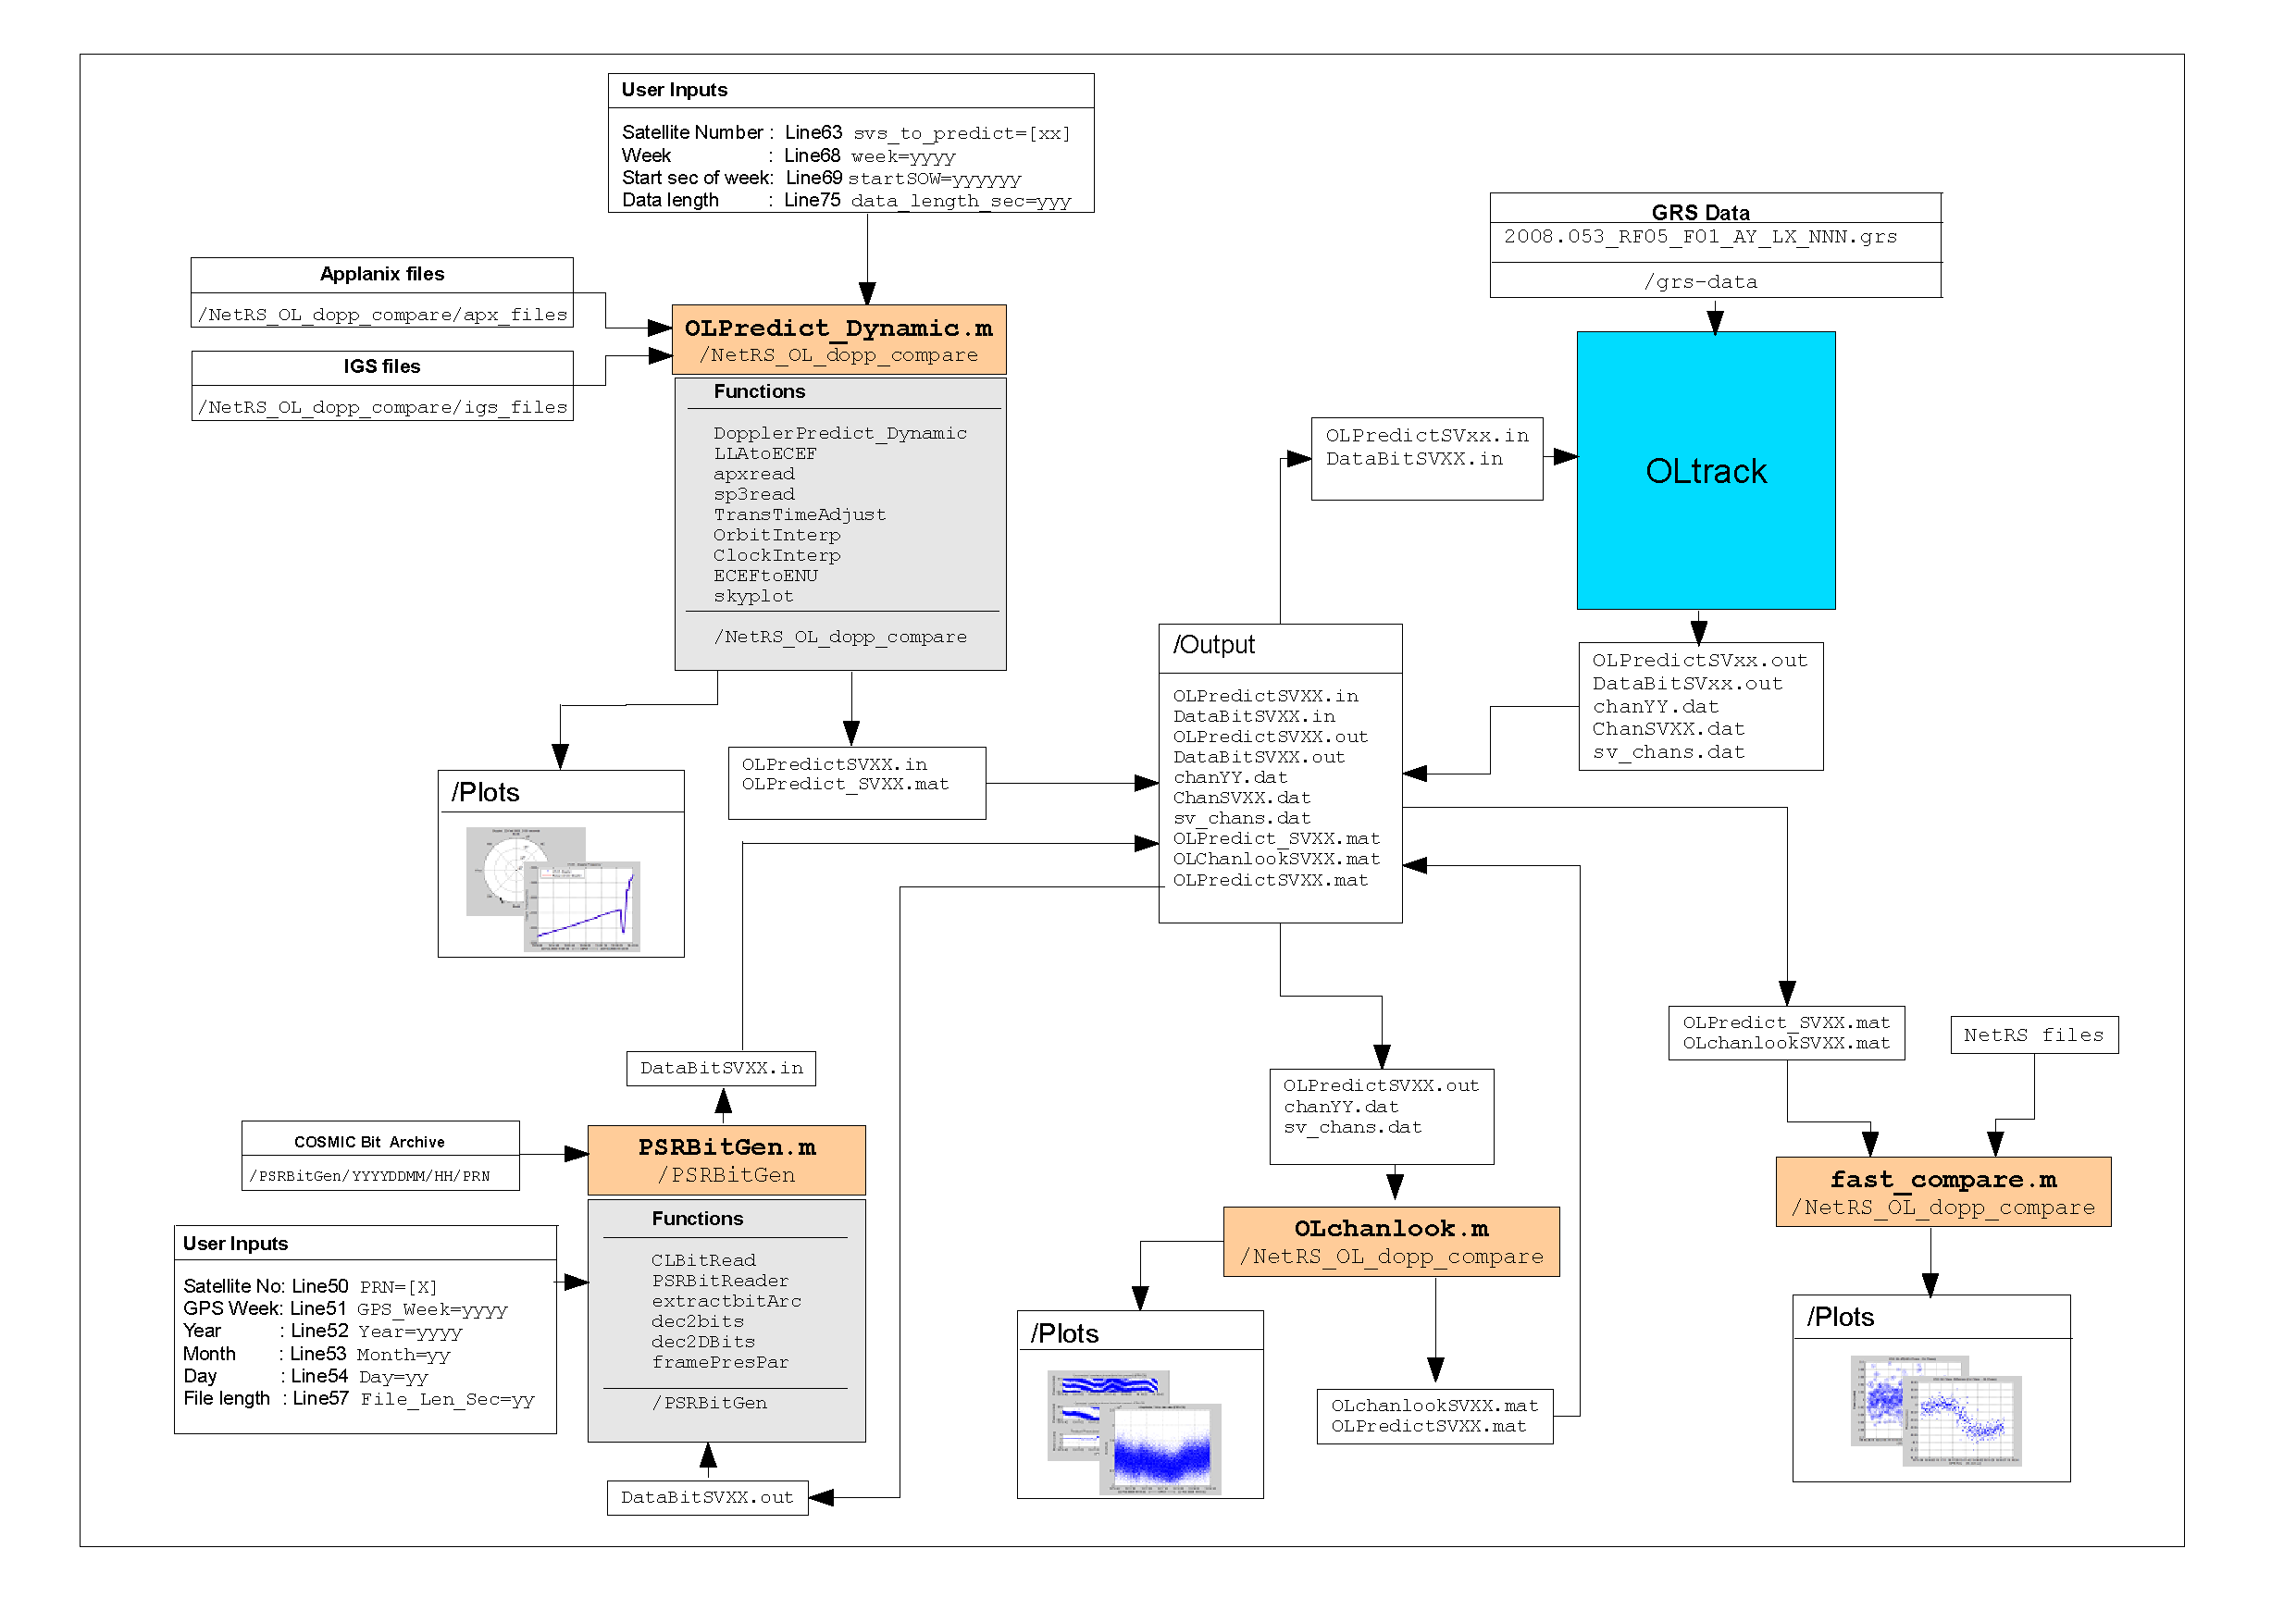
\includepdf[pages=1]{Lin-OL-track-chart.pdf}
%-----------------------------------------------------------------
% 1 Main Program Names(file path)

\section{Main Program Names(file path)}
\renewcommand\theenumi{\roman{enumi}}
\begin{enumerate}
\item OLtrack (/ OLtrack)
\item OLPredict\_Dynamic.m (/ NetRS\_OL\_dopp\_compare)
\item PSRBitGen.m (/ PSRBitGen)
\item OLchanlook.m (/ NetRS\_OL\_dopp\_compare)
\item fast\_compare.m (/ NetRS\_OL\_dopp\_compare)
\end{enumerate}
%-----------------------------------------------------------------
% 2 Compiling the OLtrack
\section{Compiling the OLtrack}
{\indent\indent} The OLtrack requires Linux OS with g++ library to compile. The program includes a "makefile" which holds instructions for all "makes".  Also, the compiler options and code paths are written into this file. The makefile is placed in /OLtrack directory. To compile the program, go to this directory and type\\\\
{\fontfamily{pcr}\selectfont make}\\\\
If the compiling is successful this massage appears\\\\
{\fontfamily{pcr}\selectfont ---- Build Complete ----}\\\\
and the executable file \emph{OLtrack} is created into the same directory.


% 2 Using the PSR

\section{Using the OLtrack}
{\indent\indent}  OLtrack is designed to track both setting and rising occultations. So, it can be run with two different options,\\\\
(1) Forward tracking option (default): {\indent} {\fontfamily{pcr}\selectfont ./OLtrack -f}\\
(2) Backward tracking option: {\indent\indent\indent} {\fontfamily{pcr}\selectfont ./OLtrack -b}\\\\
The OLtrack accepts the file name and file number of a GRS file. The filename entered by the user is a truncated version of the original that drops all characters after the standard "AX\_LY" or "CHX\_LY" ending, where X is (0,1,2) for the three different channels and Y is (1,2) for L1 or L2 band.\\\\
Example:\\
{\indent\indent} {\fontfamily{pcr}\selectfont Filename: /media/OCCevent/2008.053\_RF05\_F01\_A2\_L1}\\
{\indent\indent} {\fontfamily{pcr}\selectfont Msec per file: 399001}\\
{\indent\indent} {\fontfamily{pcr}\selectfont First file number: 1}\\
{\indent\indent} {\fontfamily{pcr}\selectfont Last file number: 5}\\\\
This will cause the OLtrack start with file:\\\\
{\indent\indent} 2008.053\_RF05\_F01\_A0\_L1\_399001\_399001.grs\\\\
which is the File 1 and the tracking will continue until the end of the File 5. In backward tracking mode tracking starts with the first file and goes backward, so the first file number must greater than or equal to the last file number. If the file is opened successfully this message appears on the screen,\\\\
{\fontfamily{pcr}\selectfont File 1:/media/OCCevent/2008.053\_RF05\_F01\_A2\_L1\_399001\_399001.grs}\\\\
and if the file could not find in the given directory it gives the following error message.\\\\
{\fontfamily{pcr}\selectfont Unable to Open file!}\\\\
In backward tracking, the program is not able to track bacdwardly more than one satellite at the same time. So, after CL tracking ended the program wants a user input to choose a channel then starts backward OL tracking only for this channel.\\\\
The OLtrack outputs files to:\\\\
{\indent\indent}/Output\\\\
This is the location which the OLtrack will search for OL input files (OLPredictSVXX.in, DataBitSVXX.in) and put output files (OLPredictSVXX.out, DatabitSVXX.out, chanYY.dat, sv\_chans.dat).
%----------------------------------------------------------------
% 3 Using OLPredict.m

\section{Using OLPredict.m}
The main user inputs will be the
\begin{enumerate}
\item SV number
\item GPS week
\item MSOW (starting millisecond of the week)
\item prediction length in seconds
\item name of the applanix position and velocity file
\end{enumerate}
{\indent\indent}It requires the presence of the IGS orbit file and Applanix (apx) position and velocity file in the same directory, or in an added path. The best course of action is to add the following directories to the path:\\
\begin{enumerate}
\item \textbackslash NetRS\_OL\_dopp\_compare\textbackslash apx\_files
\item \textbackslash NetRS\_OL\_dopp\_compare\textbackslash igs\_files
\end{enumerate}

OLPredict will create OLPredictSVXX.in, which is placed in the output folder for OL tracking. It also creates plots of elevation, predicted doppler frequency, and airplane trajectory (if using less than 1ms spacing, because otherwise there is too much data and we run out of memory). OL-Predict.m will produce a warning if the prediction period is too long, usually between 39 and 45 minutes, because of the discontinuities produced in the velocity measurements. It also saves some data for later use by the \emph{fast\_compare.m} program under a file named \emph{OLPredict\_SVXX.mat}. This program can handle batch requests.
%-----------------------------------------------------------------
% 4 Using PSRBitGen.m

\section{Using PSRBitGen.m}
PSRBitGen.m requires the presence of a file from CL tracking to operate. It operates by extracting bits from the COSMIC bit archive (bitArc) starting with the given z-count and ending after a user defined amount of time which is governed by the length of the prediction from \emph{OLPredict.m}. Then, it compares the archive bits with CL bits and changes the sign of the bits, if needed. Substantial error messaging will alert user to any problems. If a data bit file is not found, it may indicate the user did not add the directory to path, or the bitArc does not contain the data. The bitArc files must be in the same directory and in the format given in Section 9. The program will create \emph{DataBitSVXX.out} place in the output directory for OL tracking. This program can handle batch requests.\\
User must define:
\begin{enumerate}
\item PRN
\item GPS\_Week
\item Year
\item Month
\item Day
\item starting z-count
\item prediction length
\end{enumerate}
%-----------------------------------------------------------------
% 5 Using OLchanlook.m

\section{Using OLchanlook.m}
{\indent\indent} OLchanlook will extract OL and CL data, creating plots of residual phase and amplitude, as well as reducing the data over 20ms. User must define SV and type of occultation(rising or setting). It also saves some data for later use by the \emph{fast\_compare.m} program under a file named \emph{OLchanlookSVXX.mat}. This program can handle batch requests.
%----------------------------------------------------------------
% 6 Using fast_compare.m

\section{Using fast\_compare.m}
This is the final step in comparing the products from OL tracking to NetRS data.The user must have the appropriate NetRS file in the current directory. The user must also define the following:
\begin{enumerate}
\item SV
\item type of occultation
\item NetRS rinex filename
\item name of saved file from OLPredict 
\item name of saved file from OLchanlook
\end{enumerate}
This will produce comparison plots of the phase from OL tracking, and the phase as recorded by the NetRS.
%----------------------------------------------------------------
% 7 OL tracking flow

\section{OL tracking flow}
\begin{enumerate}
\item Run OLtrack to see which SV's are acquired, if some are, let it run long enough to write at least one batch z-count of databits to the data bit output file(DataBitSVXX.out).
\item Run OLPredict.m
\item Run PSRBitGen.m
\item Run OLtrack
\item Run OLchanlook.m
\item Run fast\_compare.m
\end{enumerate}
%----------------------------------------------------------------
% 8 Input-Output Files

%OLPredictSVXX.out
\newpage
\section{Input-Output File Formats}
\begin{table}[H]
\caption{OLPredictSVXX.out   Nx11}
\centering
\begin{tabular}{l l}
\hline\hline
Column Number&Variables \\[0.5ex]
\hline
1&GPS Week\\
2&GPS millisecond of the week\\
3&Header milliseconds of the week(same as the (2))\\
4&Doppler Frequency (Hz)\\
5&Inphase (V)\\
6&Quadrature (V)\\
7&Residual phase (cycles)\\
8&NCO phase (cycles)\\
9&Data bit\\
10&Samples per cycle\\
11&Edge index\\
\hline
\end{tabular}
\label{tab:OLpredictOUT}
\end{table}
%chanYY.dat
\begin{table}[H]
\caption{chanYY.dat   Nx14}
\centering
\begin{tabular}{l l}
\hline\hline
Column Number&Variables\\[0.5ex]
\hline
1&Doppler frequency (Hz)\\
2&Code rate (Hz)\\
3&Carrier phase (cycles)\\
4&Inphase Early correlator (V)\\
5&Quadrature Early correlator (V)\\
6&Inphase Promt correlator (V)\\
7&Quadrature Promt correlator (V)\\
8&Inphase Late correlator (V)\\
9&Quadrature Late correlator (V)\\
10&Promt inphase avarage\\
11&Long count(0,1,...,N)\\
12&Edge index\\
13&z-count\\
14&GPS millisecond of the week\\
\hline
\end{tabular}
\label{tab:chan}
\end{table}\newpage
%sv_chans.dat 
\begin{table}[H]
\caption{sv\_chans.dat   Nx2}
\centering
\begin{tabular}{l l}
\hline\hline
Column Number&Variables\\[0.5ex]
\hline
1&Channel Number\\
2&Satellite Number\\
\hline
\end{tabular}
\label{tab:svchan}
\end{table}

%OLPredict_SVXX.mat
\begin{table}[H]
\caption{OLPredict\_SVXX.mat}
\centering
\begin{tabular}{l l}
\hline\hline
Variables&Definition \\[0.5ex]
\hline
sp3\_filename&IGS filename(ex. igs14675.sp3)\\
svs\_to\_predict&Satellites to predict\\
CarrierPhase&Carrier Phase (cycles)\\
Range&Distance between the SV and receiver (m)\\
gps\_sow\_vec&GPS seconds of the week\\
GPS\_SOW\_Range&same as the gps\_sow\_vec\\
\hline
\end{tabular}
\label{tab:OLpredictMAT1}
\end{table}\\
%OLPredictSVXX.mat
\begin{table}[H]
\caption{OLPredictSVXX.mat}
\centering
\begin{tabular}{l l}
\hline\hline
Variables&Definitions \\[0.5ex]
\hline
GPS\_Wk&GPS week\\
GPS\_MSOW&GPS milliseconds of the week\\
Header\_MSOW&same as GPS\_MSOW\\
Freq&OL tracking Doppler frequency (Hz)\\
I&Correlator Inphase\\
Q&Correlator quadphase\\
PhiResidual&Residual phase (cycles)\\
PhiNCO&NCO Phase (cycles)\\
DataBit&Data bits\\
SamplesPerCycle&Samples per Cycle \\
EdgeIndex&Edge index\\
\hline
\end{tabular}
\label{tab:OLpredictMAT2}
\end{table}\\
%OLchanlookSVXX.mat
\begin{table}[H]
\caption{OLchanlookSVXX.mat}
\centering
\begin{tabular}{l l}
\hline\hline
Variables&Definitions \\[0.5ex]
\hline
Doppler\_CL&CL Tracking Doppler frequency (Hz)\\
Freq&OL tracking Doppler frequency (Hz)\\
PhiResidual&Residual phase (cycles)\\
GPS\_MSOW&GPS milliseconds of the week\\
PRN&PRN number\\
CorrCorrectPhaseR&Reduced corrected phase (cycles)\\
PhiNCO&NCO Phase (cycles)\\
GPS\_Wk&GPS week\\
gps\_sd\_vec&GPS seconds of the day\\
gps\_sd\_vecR&Reduced GPS seconds of the day\\
\hline
\end{tabular}
\label{tab:OLchanlookMAT}
\end{table}\\
%OLPredictSVXX.in
\begin{table}[H]
\caption{OLPredictSVXX.in  (binary file)}
\centering
\begin{tabular}{l l}
\hline\hline
Size&Variables \\[0.5ex]
\hline
unsigned short&GPS week\\
unsigned long&GPS seconds of the week\\
double&Predicted Doppler frequency[1000] (Hz)\\
\hline
\end{tabular}
\label{tab:OLpredictIN}
\end{table}

\begin{table}[H]
\caption{DataBitsSVXX.in and DataBitsSVXX.out (binary files)}
\centering
\begin{tabular}{l l}
\hline\hline
Size&Variables \\[0.5ex]
\hline
unsigned long&Z-count\\
short&Data bits[300] \\
\hline
\end{tabular}
\label{tab:databits}
\end{table}

\noindent{\large\bf COSMIC Data Bit Files}\\
Data files are created in the following format:\\\\
/\textless YYYYMMDD\textgreater /\textless HH\textgreater /\textless PRN\textgreater cdbs\_ \textless PRN\textgreater\_ \textless frameStart\textgreater\_ \textless sfMask\textgreater\_ \textless sfParityMask\textgreater\_ \textless CN0\textgreater\_ \textless hostNumber\textgreater .bin\\
\begin{itemize}
\item {\bf PRN} -Satellite PRN (not SV number)
\item {\bf YYYYMMDD} -Year,Month,Day
\item {\bf HH} -Hour
\item {\bf hostName} -As obtained from gethostname function call(cdbs)
\item {\bf hostNumber} - 01-10(cdbs01-cdbs10)
\item {\bf frameStart} - GPS time for frame 1 start(time in seconds since GPS epoch)
\item {\bf sfMask} - Binary mask of subframes in file(bit0=sf1,bit4=sf5).0=not present,1=present.
\item {\bf sfParityMask} - If bit is set, then that subframe passed parity. 
\item {\bf CN0} - Avarage Carrier to Noise ratio for that frame
\end{itemize}\\
The data file is defined by the following structure:\\\\
char hostName[8];\\
UINT8 prn;\\
UINT8 CN0;\\
UINT8 sfMask;\\
UINT8 sfParityMask;\\
UINT32 frameStart;\\
UINT32 subframe1[10]\\
UINT32 subframe2[10]\\
UINT32 subframe3[10]\\
UINT32 subframe4[10]\\
UINT32 subframe5[10]\\
(216 bytes)\\\\
An example file name:\\\\
/20050521/10/02/cdbs\_02\_0800708070\_1f\_1f\_49\_01.bin\\\\
This file indicates cdbs01 was tracking PRN02 on 21 March 2005 with a CN0 of 49dBHz during hour 10 (GPS time). All subframes were present and all parity passed.
\newpage
\section{Codes}
\subsection{Doppler prediction}
\VerbatimInput{./code/DopplerPredict_Dynamic.m}
\subsection{OL Doppler Prediction}
\VerbatimInput{./code/OLPredict_Dynamic.m}
\subsection{OL Phase}
\VerbatimInput{./code/OLchanlook.m}
\subsection{NetRS-OL Excess Phase Compare}
\VerbatimInput{./code/fast_compare.m}
\end{document}